\subsection{ボタンを使って LED をつけてみよう (2)}
HSPスクリプトエディタで\textasciitilde /03/button\_led2.hspを読み込み実行してください。前のプログラムではボタンを押している間LEDがつきましたが、今度はボタンを押すたびにLEDのON/OFFが変わります。\\

\begin{lstlisting}[caption=button\_led2.hsp,label=button_led2.hsp]
#include "hsp3dish.as"		<#blue#;スクリプトの設定を読み込む#>
#include "rpz-gpio.as"		<#blue#;スクリプトの設定を読み込む#>

 gpio 17, 0
 gpio 18, 0
 gpio 22, 0
 gpio 27, 0
	
 redraw 0		<#blue#;画面更新(仮想画面に描画)#>
 font "",30		<#blue#;フォントサイズを決める#>
 pos 20,20		<#blue#;文字の位置を決める#>
 mes "赤いボタンを押して、LEDをつけたり消したりできるよ"	<#blue#;表示する文字を決める#>
 redraw 1		<#blue#;画面更新(実際の画面に描画)#>

 ima_btn = 1		<#blue#;今ボタンを押しているかどうかの変数#>
 mae_btn = 1		<#blue#;前回はボタンを押しているかどうかの変数#>
 led = 1		<#blue#;LEDを光らせるかどうか決める変数#>

*hata
  ima_btn = gpioin(5)
  if ima_btn = 0{		<#blue#;今押されているとき#>
    if mae_btn = 1{	<#blue#;前は押されていなかったとき#>
      led = 1 - led	<#blue#;LEDの消灯を切り替える#>
    }
  }
    gpio 22, led		<#blue#;GPIO22をつけるか消すかする#>
  mae_btn = ima_btn	<#blue#;今の状態を前回の状態とする#>

  await 10
  goto *hata
\end{lstlisting}

ここで登場したif命令が今まで登場したif命令とは少し違うことに気が付きましたか?\\
第二回の「条件判断とは」では次のようになっていました。\\
\begin{center}
 					if 条件式 : 命令 \\
\end{center}
最初に条件式を書いて、次に条件が正しい時に実行される命令を一つだけ書きました。しかし、今回のプログラムでは次のようになっています。\\
\begin{center}
  \begin{minipage}{4cm}
    if 条件式 \{\\ \ \ 命令\\ \}
  \end{minipage}
\end{center}
どちらも条件判断をしたいときに使えるHSPのルールですが、{}を使ったif命令は、条件が正しかったときに複数の命令を書くことができます。\\
\begin{center}
  \begin{minipage}{4cm}
					if 条件式 \{\\
					  \ \ 命令1\\
					  \ \ 命令2\\
					  \ \ ...\\
					\}\\
  \end{minipage}
\end{center}
今回のプログラムではif命令の中で別のif命令とled = 1 – led という2つの命令を使うために{}を使っているわけです。\\

\begin{center}
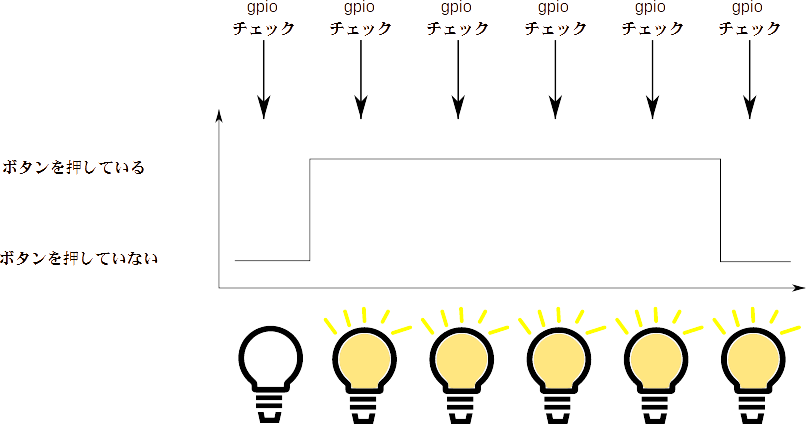
\includegraphics[width=\linewidth]{images/chap03/text03-img033.png}
\end{center}

ボタンを使ってLEDをつけたり消したりするには 工夫が必要です。「前回はボタンが押されていたかったけど今はボタンが押されている」ときのみLEDのON/OFFを切り替える必要があります。これを「変化を検出する」といいます。

LEDのON/OFFを切り替えているのは、\code{led = 1 – led}の部分です。
例えば、変数ledの中身が1だったとします。そうすると\code{led = 1 – led} は\code{led = 1 – 1} となるので変数ledは0になります。
反対に変数ledの中身が0だったとすると、\code{led = 1 – 0} となって変数ledは1になります。

このようにして0と1を交互に切り替えることで、ON/OFFの切り替えを実現しています。\\

\begin{tcolorbox}[title=\useOmetoi]
\label{button_led2_toi}
\begin{enumerate}
\item ターミナルを使ってbutton\_led2.hspのコピーを、332.hspという名前で作りましょう。\\
\fbox{\phantom{白}} $\leftarrow$できたらチェックしましょう。
\item 黒いボタン(GPIO6)でLEDが点灯するように332.hspのプログラムを変えてみましょう。\\
\fbox{\phantom{白}} $\leftarrow$できたらチェックしましょう。
\item 赤いボタン(GPIO5)でLED1(GPIO17)、黒いボタン(GPIO6)でLED3(GPIO22)が点灯するように332.hspのプログラムを変えてみましょう。\\
\fbox{\phantom{白}} $\leftarrow$できたらチェックしましょう。
\end{enumerate}
\end{tcolorbox}